% Generated by Byrne from a live model. Regenerate; do not hand-edit.
%
% NOT exported to TikZ:
%   - gradient fills
%   - clipping paths other than the page rectangle
%   - the viewport surface shading
%   - any 3D information: this is the projected figure, not the scene
%   - round-tripping back into Byrne

\tikzset{
  byrne force/.style={draw=byrneforce, line width=0.4pt, -{Stealth[length=2mm]}},
  byrne structure/.style={draw=byrnestructure, line width=0.4pt},
  byrne guide/.style={draw=byrneguide, line width=0.3pt, dashed},
}
\definecolor{byrneforce}{HTML}{C0392B}
\definecolor{byrnestructure}{HTML}{2B2B28}
\definecolor{byrneguide}{HTML}{9A9A93}
\definecolor{byrnefield}{HTML}{8E44AD}

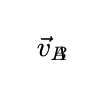
\begin{tikzpicture}
  \node[anchor=south west] at (9.878,6.703) {$\vec{v}_A$};
  \node[anchor=south west] at (9.878,6.703) {$\vec{v}_B$};
\end{tikzpicture}
